\chapter{ReLUSyn}
In this section we explain the inner workings of our tool ReLUSyn. 
We provide formal models for a \ac{DNN}s that we use to create \ac{MILP} models. 
We use a generic representation and describe the modeling of cost functions that we use to generate \ac{RFDIA}.
We then show how this allows us to identify critical inputs and find the perturbations. 
We finally explain how we map this to real systems. 
We build on the approach proposed by Fischetti et al. \cite{fischetti2017deep} where they propose a 0-1 MILP model. 
\begin{figure}
	\centering
	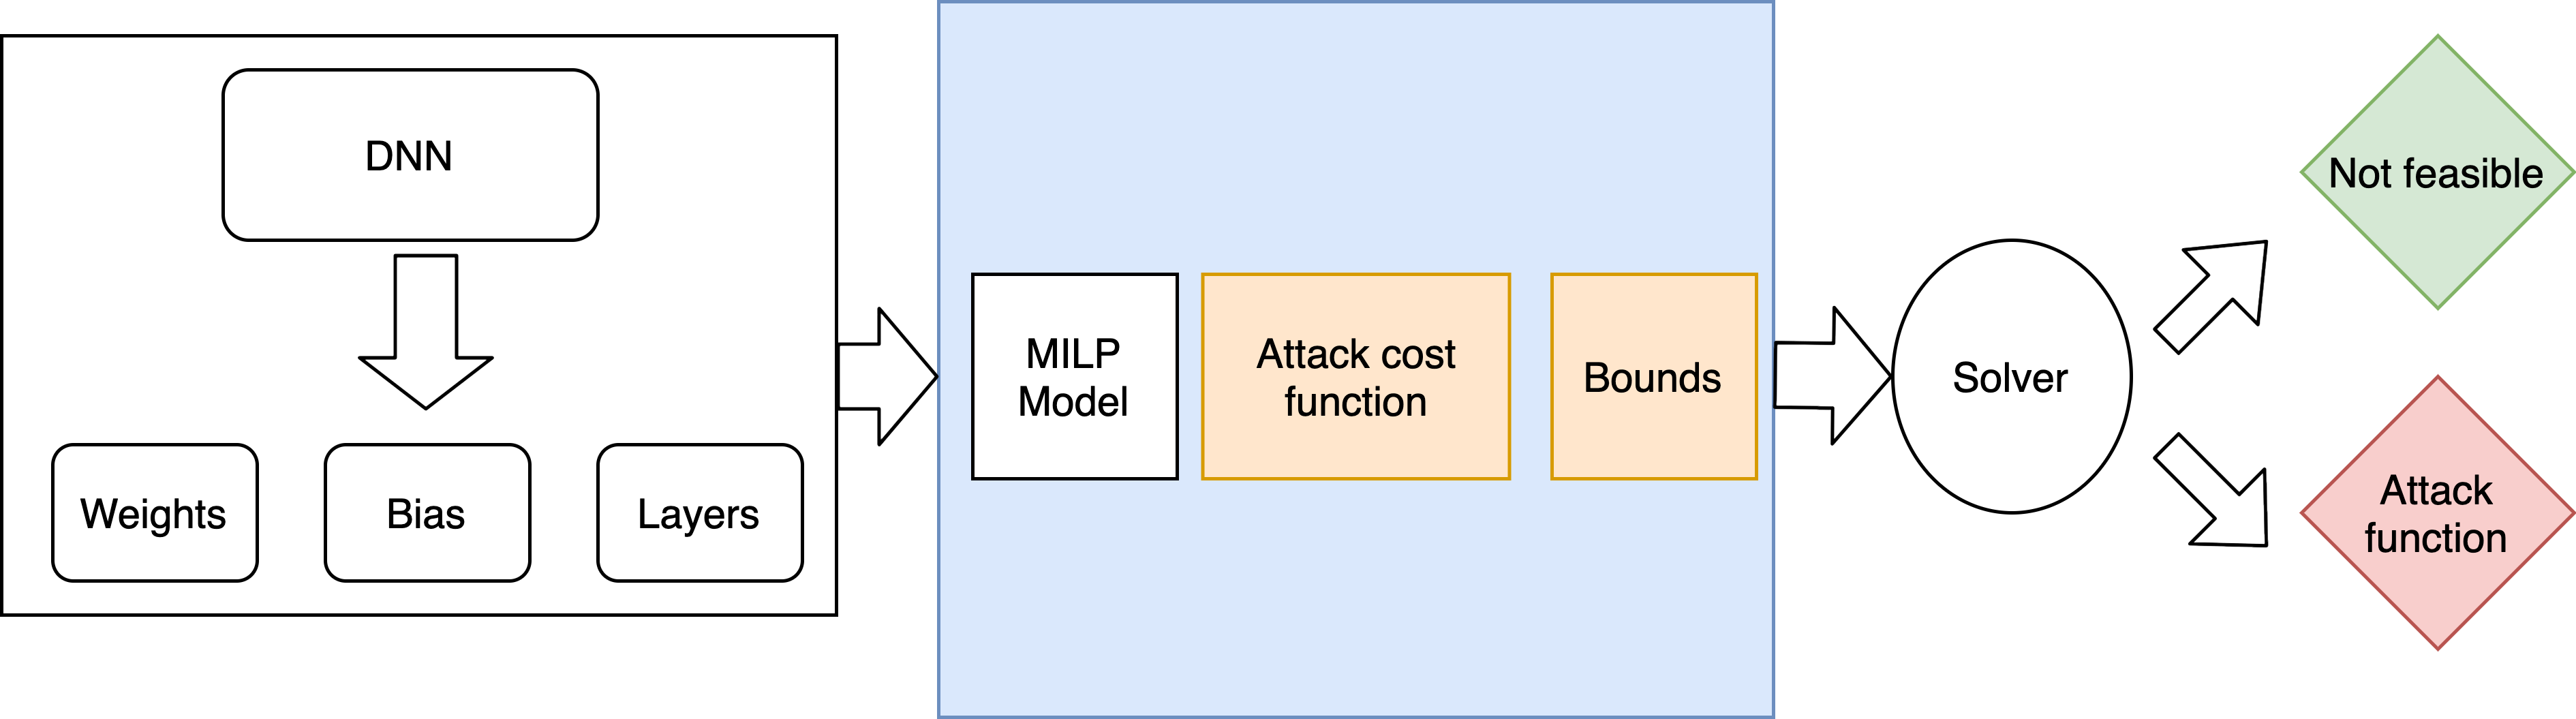
\includegraphics[scale=0.1]{Images/Methodology}
	\caption[Methodology]{The rounded boxes depict the information provided by the users and the sharp corners is the information provided by us that integrates the first layer into the solver layer.}
	\label{fig:methodology}
\end{figure}

\begin{figure}
	\centering
	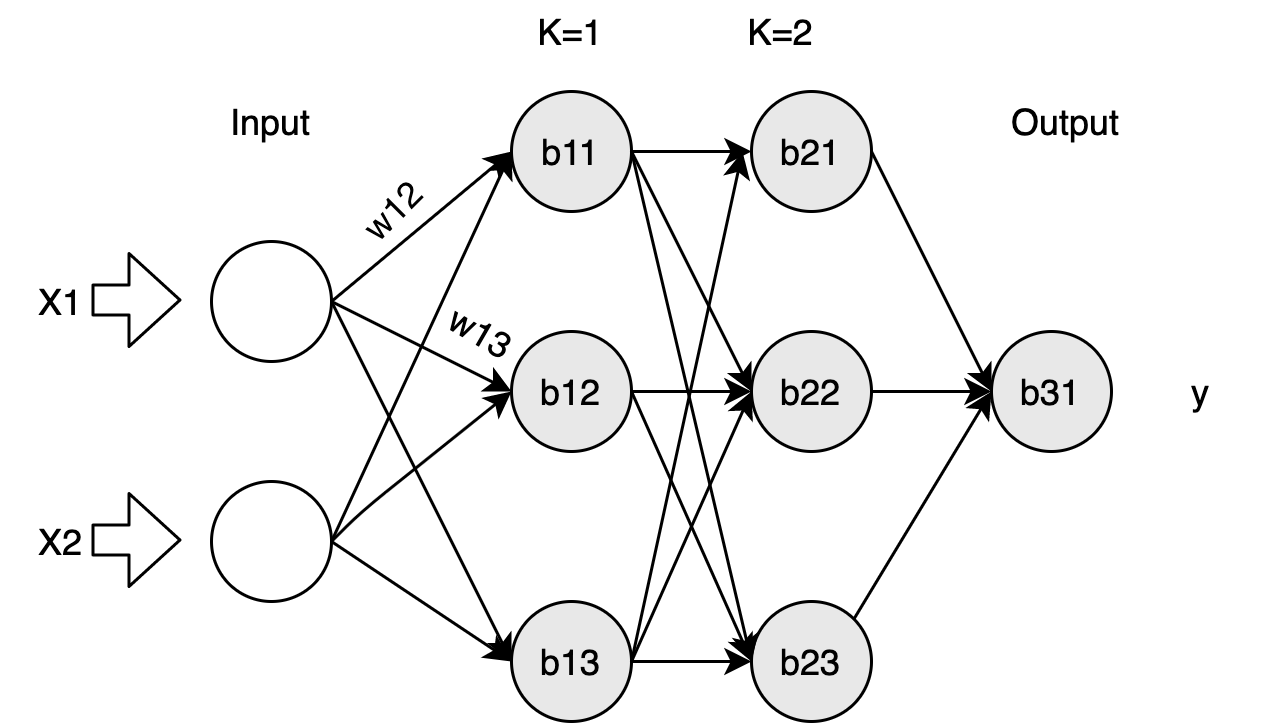
\includegraphics[width=0.7\linewidth]{Images/DNNstructure}
	\caption[DNN structure]{DNN controller structure with two hidden layers K=1,2, two inputs x1 and x2 and one output y. This is an example of a fully connected network.}
	\label{fig:dnn-controller}
\end{figure}


\section{ReLUSyn: Overview}
ReLUSyn is the technique that allows the attacker to generate \ac{RFDIA} attacks directly from the \ac{DNN} model. 
Our technique is shown in Figure 5.1.
The \ac{DNN} is made available from the systems which can be diirectly passed through ReLUSyn. 
It automatically synthesizes a \ac{MILP} model from the \ac{DNN} model which also contains the cost or objective functions. 
The cost function and bounds have a plug-gable functionality. 
Everything inside the blue box is automatically synthesized.
The orange parts can be easily changed to extend the technique for different systems and applications in the future. 
The models along with the cost functions and bounds are passed through the solver that synthesize the attacks if they exist else shows an infeasible model that implies that no attacks exist. 
\section{DNN formalism}
We follow the formalism based on the general architecture that we explain in Chapter 2. 
The \ac{DNN} controller maps the inputs that are the $x1$ and $x2$ to the output $y$ as shown in  Figure 5.2.   
We now begin with the formal modeling of the \ac{DNN}.


%Formal modeling of a DNN for later use when explaining the modeling in MILP  
The architecture can be represented as a function F defined as $F: X \rightarrow Y$ where the inputs X are mapped to the output Y and are composed of multiple layers. 
We consider \ac{DNN} to be made up of $K + 1$ layers, numbered from 0 to K.
Layer 0 does not really exist since it is the input layer of the network.
The last layer K corresponds to the output of the \ac{DNN}.
Every individual layer in the \ac{DNN} $k$ $\epsilon$ $\{0,1,....,K\}$ is made by $n_k$ nodes or neurons in the network.
Each neuron has a bias associated with it. 
Every neuron from the previous layer is connected to every neuron in the next layer. 
The neurons are labeled starting from $1$ to $n_k$ in the network. 
We denote every neuron by $NODE(i,k)$ which corresponds to $ith$ node for the layer k. 

We denote the output vector of the layer k as $F_k(x)$.
The output for every $NODE(i,k)$ denoted as $F_{ik}(k)$ where $i$ $\epsilon$ $\{0,1,....,n_k\}$ 

The output for layer 0 which is the \ac{DNN} input is represented as $F_k(0)$.
The output for every layer $k \geq 1$ the output vector is represented as  the following. 

\begin{equation}
\begin{aligned}
F_k(x) &= \upsigma(W^{k-1}x^{k-1} + b^{k-1}) \\
\end{aligned}
\end{equation}

$\upsigma$ is the abstraction for different activation functions that can be used to model the DNN. 
There are multiple types of activation functions which all come with different modeling capabilities such as ReLU ($f(x) = max {0,x}$) as shown in Figure 5.3, logistic $f(x)=1/(1+ exp(-e))$
Our tool focuses on using Rectified Linear Unit (ReLU) since it is one of the commonly used activation functions in \ac{DNN}s as Krizhevsky et al. \cite{10.1145/3065386}. 
Hence, our equation now looks  something like where, for a real vector x, ReLU(x):= max\{0,x\} (per layer).

\begin{equation}
\begin{aligned}
F_k(x) &= ReLU(W^{k-1}x^{k-1} + b^{k-1}) \\
\end{aligned}
\end{equation}

Since a network consists of multiple layers, the general \ac{DNN} representation looks like a composition function as shown below. 
\begin{equation}
	\begin{aligned}
	F(x) &= F_K \circ F_{K-1} \circ F_{K-2} ....... \circ F_1(x),    \\
	or \\
	F(x) &= F_K ( F_{K-1}( F_{K-2} .......  (F_1(x)))),    \\
	\end{aligned}
\end{equation}

This ends  our \ac{DNN} formalism. In the next section we use the formalism to create a \ac{MILP} model. 

\section{MILP Model}
To create a \ac{MILP} model, the essence lies in studying the basic scalar equation that describes the \ac{DNN} architecture. 

\begin{equation}
\begin{aligned}
y &= ReLU(w^Ty + b) \\
\end{aligned}
\end{equation}

This equation can be represented as a set of linear constraints in the \ac{MILP} model. 
To do so we use a $max$ operation that models the ReLU behavior. 

\begin{equation}
\begin{aligned}
w^Ty + b = x - s, x \geq 0, s \geq 0 \\
\end{aligned}
\end{equation}

The reason we represent it as above is to first separate the equation from it's non-linear component such that we can convert it to it's linear component. 
As the ReLU behavior is graphically explained in Figure 5.3 that the ReLU function can be broken in two parts which are the positive and the negative parts.  
To implement such behavior we define a activation variable $ac$ that imposes the logical implications. 

\begin{equation}
\begin{aligned}
ac =  1 \rightarrow x \leq 0  \\
ac =  0 \rightarrow s \leq 0  \\
ac \epsilon  \{0,1\} \\
\end{aligned}
\end{equation}

This maps to the \ac{MILP} solvers and converts them into proper linear inequalities. 
The final \ac{MILP} model looks of the form
\begin{equation}
\begin{aligned}
& \underset{}{\text{min/max}}
& &  \sum_{k=0}^{K} \sum_{i=i}^{n_k}F_{jk}(x)   + \sum_{k=0}^{K} \sum_{i=i}^{n_k}F_{jk}(z)  \\
\end{aligned}
\end{equation}
%ReLU
ReLU constraints
\begin{equation}
\begin{aligned}
& \text{subject to} & &  \sum_{j=0}^{n_k} w_{ij}^{k-1}x_{j}^{k-1} + b_i^{k-1} = x_i^k - s_i^k  \\
& & & x_i^k \geq 0, \\
& & & s_i^k \geq 0 \\
& & & ac_i^k  \epsilon  \{0,1\} \\
& & & ac_i^k  =  1 \rightarrow  x_i^k \leq 0  \\
& & & ac_i^k =  0 \rightarrow s_i^k  \leq 0   \\
\end{aligned}
\end{equation}
Upper and lower bounds for range analysis
%Lower and upper bounds on the model
\begin{equation}
\begin{aligned}
& & & lb \geq x_i^k \geq up, \\
& & &  lb \geq s_i^k \geq up \\
& & & lb \geq z_i^k \geq up, \\
\end{aligned}
\end{equation}

We have divided our \ac{MILP} model in three main parts. 
Equation 5.7 represents the cost functions that are to be minimized and maximized.
These cost functions depend on different applications and requirements.  
We will show in the next section how we model cost functions for \ac{RFDIA}
attack synthesis. 

Equations 5.8 represents the ReLU modeling for each layer in the network. 
We showed in Equation 5.6 how we can represent ReLU units as a set of linear constraints in \ac{MILP} solvers. 
We expand on it and apply it to all the layers in the modeling. 

Equations 5.9 add lower bounds ($lb$) and upper bounds ($up$) in the  model for different variables that we will  require to add limits to our search space.  











\begin{figure}
	\centering
	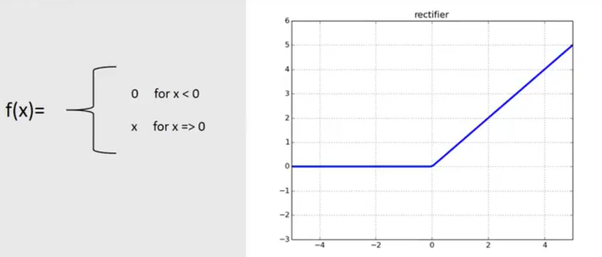
\includegraphics[width=0.7\linewidth]{Images/ReLUbreakdown}
	\caption{ReLU can be broken down into two linear units as shown in the figure for x $<$ 0 and x $\geq$ 0. This allows us to easily map the DNN equations in MILP models by breaking down the non-linearity inducing function.}
	\label{fig:relubreakdown}
\end{figure}

\section{Building the model}
\label{section:attacks}
%This section focuses on how we build the model using MILP and some background insights about DNN along with that. 
\tool comes with automated attack synthesizers for Artificial Pancreas System, Aircraft Collision Avoidance systems ACAS Xu and Horizontal CAS. %Writing a new attack synthesizer into \tool boils down to defining the attack model as a function that can be easily plugged in our framework.
As an example, we use a toy Artificial pancreas system (toyAPS) and then explain APS. A toyAPS as shown in Figure 5 consists of two sensor inputs that predict the amount of insulin as the output at some time $t$. 
\begin{figure}
	\centering
	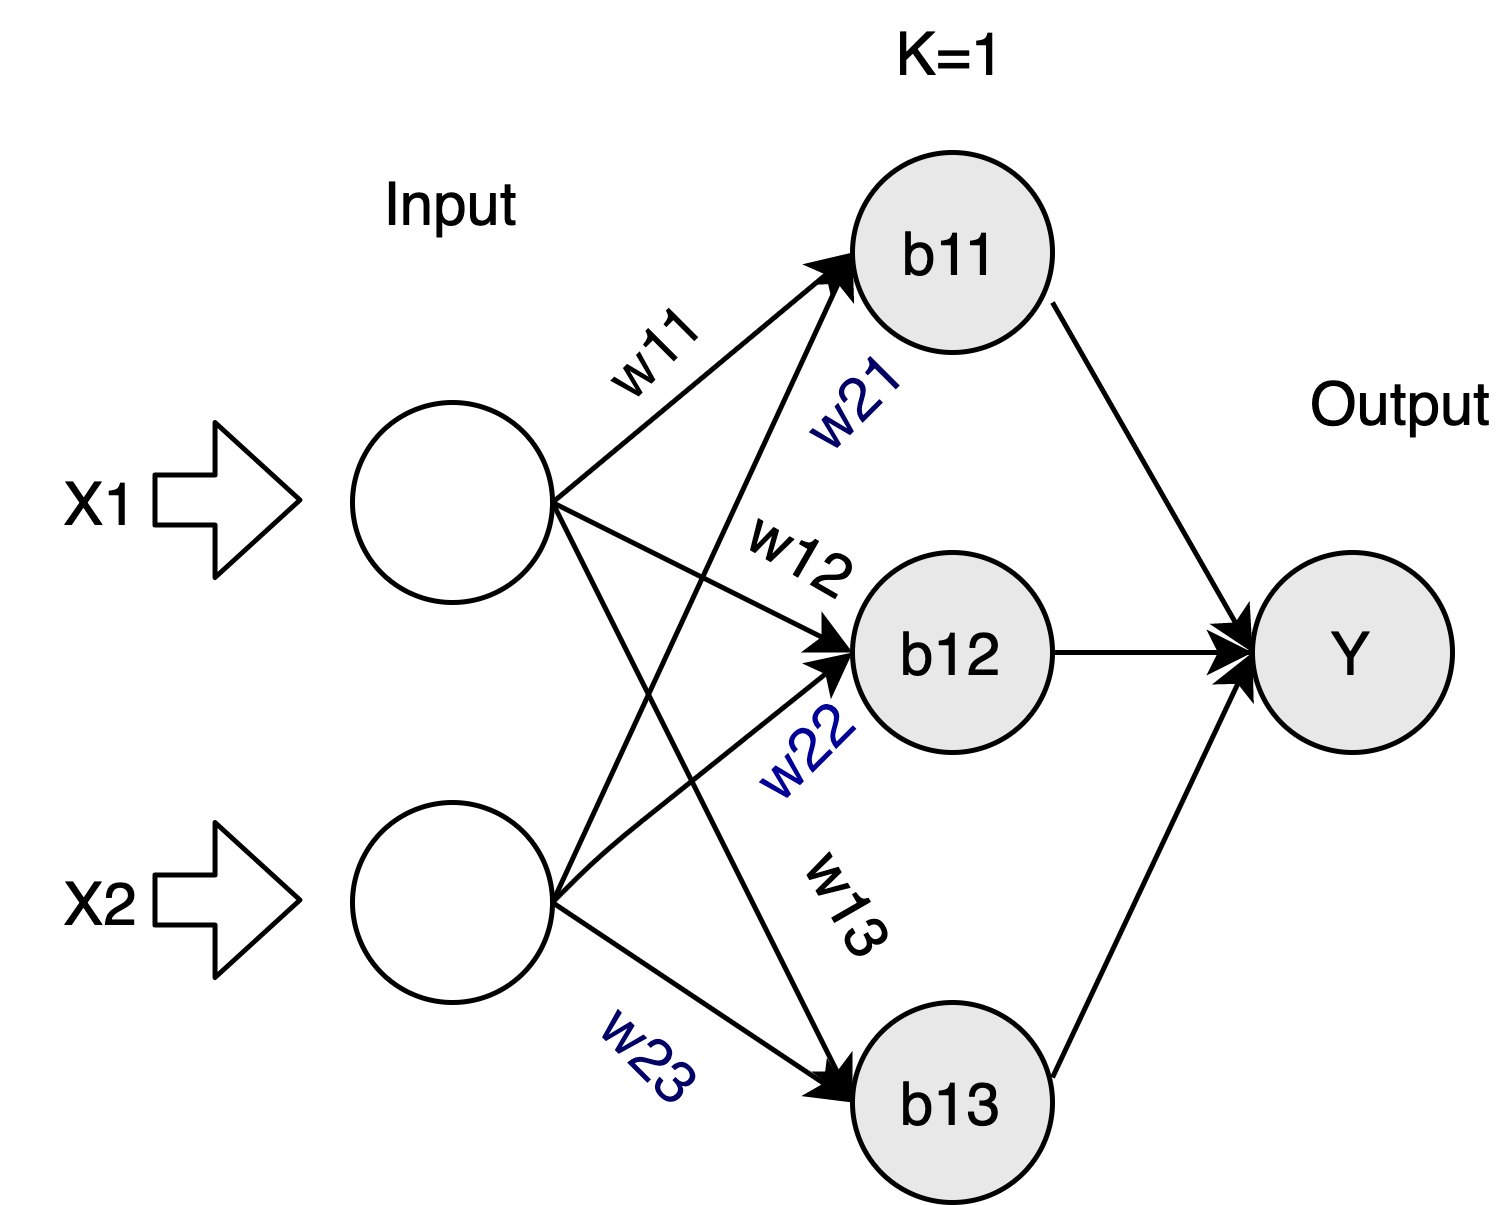
\includegraphics[width=0.7\linewidth]{Images/ToyAPS}
	\caption[A ToyAPS]{A ToyAPS that takes in two inputs which we consider as the sensor values from the human. It predicts the amount of insulin to be injected at some time based on the sensor inputs.}
	\label{fig:toyaps}
\end{figure}


\begin{algorithm}
	%\DontPrintSemicolon % Some LaTeX compilers require you to use \dontprintsemicolon    instead
	\KwIn{ weight, bias, num\_layers, num\_neurons}
	\KwOut{input, layer\_output, ReLU\_output}
	Take the weight, bias, number of layers and number of neurons per layer. \\
	
	\textbf{Model}, \linebreak
	%\renewcommand{\labelenumi}{(\Roman{enumi})}
	%\begin{enumerate}[noitemsep,nolistsep]
	%\item
	(I) For every  layer,  $expr = input * weight + bias$
	\linebreak 
	defining the linear expression
	\linebreak
	$layer\_output = expr$
	\linebreak
	%\item 
	(II) Define the non-linear activation function 
	\linebreak 
	\qquad Constraint: $ReLU(x) = max (0,x)$
	\linebreak
	(III) Adding non-linearity to every layer,
	\linebreak
	Constraints: $ReLU\_output = ReLU(0, layer\_output)$\\, 
	Repeat Step 2 until all layers are modeled 
	\linebreak
	$num\_layers < = 0$   $ \&\& $ 
	$ num\_neurons < = 0 $.
	
	\caption{Modeling neural network in MILP}
	\label{algo:b}
\end{algorithm}


The system can be represented as a MILP model through pseudo-code in Algorithm 1. This converts the neural network structure into a set of linear equations that can be mapped directly into a back-end MILP solver (we use Gurobi). %For our work we model our networks in Gurobi. 

\begin{align*}
Y &=  ReLU(Wx + b) ...... (4)
%Y &= ReLU(w_{11} x_1 + b_{11}  + w_{12} x_1 + b_{12} + w_{13} x_1 + b_{11}   )   \\
\end{align*}
The above equation represents the toyAPS. We convert the equations above into a MILP model as shown in Algorithm 1. Every layer is initially modeled as a linear equation. The activation function is represented as piecewise linear. Our approach will work for any representation of a piece-wise linear function. However, in our work we specifically focus on ReLU as explained in the problem formulation section. 
\section{Modeling cost functions for attacks}
\label{section:costfunction}
%Why is modeling cost function important
After representing the pictorial representation of a network as shown in Figure 5 to Algorithm 1, the next step is to model the cost or objective function. The cost function is what decides on the smallest perturbations of the inputs for generating a ripple. 

In our toyAPS we have two inputs $x_1$ and $x_2$ that map to an output $y$. To conduct \attack the goal is to change the inputs in a way that the alarms are not triggered and yet it leads to an output change. These small changes lead the system to end up in a bad state eventually. In toyAPS, every small increase is a bad consequence of the system. Since the output determines the amount of insulin to be injected inside the body, small increases in the output can cause the diabetic patient harm \cite{ZHANG2019403} and can lead to cancer. 
Therefore in toyAPS the attacker's goal is to change the output to $y'$, where $y' = y + a$. $a$ is some constant. %She needs to find the deviations in the input that would help her to change the outputs. 
However, the catch here is that the inputs perturbations should be very small such that the new input now provides her the output $y'$.  The reason she wants the input perturbations to be small is that there are accompanying neural networks that determine the upper and lower bounds for inputs and outputs at every stage. The reason for these accompanying networks is to ensure the patients' safety as explained in Section IV.%Hence, we have to minimize the perturbations. 
%This paragraph is explaining the subtlety of how we model our inputs for minimizing the perturbations. 
%We are hence minimizing the perturbations and not the inputs directly. Since minimizing the inputs directly will provide us with the smallest set of inputs that cause a deviation in the output. However, we want the smallest possible perturbations from the original image that change the output by the amount we want it to deviate. To find the smallest perturbations, we introduce a new variable delta for every input in the system. The new input is the addition of the original value and the minimized delta that ReLUSyn produces. 

Algorithm 1 describes the process of modeling a neural network in a MILP format. It does not consist of the cost function since the function will be different for systems depending on what the attacker wants to minimize and/or maximize. We model the objective function by introducing a new variable called $input\_delta$. Hence now the equation (1) in this section can be redefined as:

\begin{align}
Y &=  ReLU(W(x + \bigtriangleup  x ) + b) ...... (5)
\end{align}

%The new cost modeling adds one layer of extension to our previous algorithm which is the objective function. Modeling any DNN can be done in the way presented in Algorithm 1 so long the activation function can be described as piecewise linear. 
%\smi{for MILP, this is only true if the activation function is piecewise linear}.
Algorithm 2 shows how to include the cost functions for different attacks as a part of the MILP model. The cost function can be changed based on the attack requirements. 
\begin{algorithm}
	%\DontPrintSemicolon % Some LaTeX compilers require you to use \dontprintsemicolon    instead
	\KwIn{ weight, bias, num\_layers, num\_neurons}
	\KwOut{input, input\_delta layer\_output, ReLU\_output,}
	Take the weight, bias, number of layers and number of neurons per layer. \\
	
	\textbf{Model}, \linebreak
	%\renewcommand{\labelenumi}{(\Roman{enumi})}
	%\begin{enumerate}[noitemsep,nolistsep]
	%\item
	(I) For every  layer,  $expr = input * weight + bias$
	\linebreak 
	defining the linear expression
	\linebreak
	$layer\_output = expr$
	\linebreak
	%\item 
	(II) Define the non-linear activation function 
	\linebreak 
	\qquad Constraint: $ReLU(x) = max (0,x)$
	\linebreak
	(III) Adding non-linearity to every layer,
	\linebreak
	Constraints: $ReLU\_output = ReLU(0, layer\_output)$\\, 
	Repeat Step 2 until all layers are modeled 
	\linebreak
	$num\_layers < = 0$   $ \&\& $ 
	$ num\_neurons < = 0 $.\\
	
	\textbf{Cost/Attack Function} \linebreak
	$Minimize $  $input\_delta$
	\caption{Modeling neural network in MILP}
	\label{algo:b}
\end{algorithm}

If there are two inputs as in our toyAPS, we can either try to minimize the delta values for both the inputs or only one of the inputs. The reason it is important to understand this is because, in general, APS, there are inputs that come from two different sensors as explained in the motivating example section. %The first sensor is attached to the back of the patient that captured the blood-glucose levels of the patient and the second input is from the insulin pump to get the measure of the insulin level in the pump.
The attacker might want to make changes to only one of the sensor readings. Hence, considering different scenarios, we can minimize the values depending on which input we are interested in conducting an FDI attack. 

\section{Finding critical inputs}
In our running example of APS, in reality, there are 74 inputs collected from two sensors every five minutes. The goal of the attacker is to locate the critical inputs such that they can conduct FDI at the right time. To do so, as described in the previous two sections, the tool can be used to chose the index of inputs to be perturbed. 

If the attacker wants to locate one input that on perturbing by the smallest amounts can lead to the output change, they can specifically choose those inputs for conducting \attack.

%Depending on the attack model of the attacker, they can choose input(s) they are interested in finding the minimum perturbations for. We have implemented a framework that allows the users to pass the input index for inputs to be perturbed as a parameter. We will show this in the Evaluation section in more detail. 
\label{section:cost function}
\section{Synthesizing attacks}
The final part is synthesizing the inputs that can be used to conduct \attack without triggering any alarms in the system. To do so we introduce the final constraints that put lower and upper bounds on the output of the networks. This is important for the optimization to return useful results. The reason the optimization approach wins here is that if we provide the proper constraints it gives us results in less than a second per attack. This precise modeling is the secret sauce that scales up our technique significantly and provides us \attack based on the scenario. Due to the proper ranges, the state space is handles well by our technique and does not result in blowups. 
%\aarti{Should I add more here and also the algorithm for the synthesizing attack aspect?}              

